\documentclass[letterpaper,10pt,twocolumn]{article}
\usepackage{graphicx}

\title{Development of traces generator for ARM processor}
\author{Jeoffrey Spinoza and Surenkumar Nihalani}

\begin{document}
\maketitle


\section{Abstract}
Memory hierarchy is an important factor in systems design. In order to inform decisions as to what hardware improvements can be made to to a computer architecture, it is necessary to simulate execution of practical programs on that architecture and obtain timing data. There is no way to define the memory hierarchy and simulate the structure of CPU and measure the time. We do have simulators that allow us to define the model, take the program as input and calculate the execution time of the program. For such simulators, you need assembly instruction and the simulator doesn't execute the code, it just simulates the access and write times. Hence, it is a code inspection software. We need to run the program and get all the instructions executed. once, we have the instructions, we can use the timing simulator to find out the metrics of performance of the cpu. The purpose of our software is to extract the list of executed instructions with register accesses and memory access from the emulator for input into timing simulators. Our focus is to develop such a tool for an ARM emulator.
\subsection{Subsection}
Vestibulum congue fringilla mauris, eu aliquet libero pretium nec. Nulla facilisi. Morbi pellentesque sollicitudin ultricies. Nam tristique nulla convallis quam auctor eu euismod nulla tempor. Donec consectetur eleifend semper. Donec ut turpis neque, ac gravida quam. Suspendisse a quam sed libero scelerisque ullamcorper in sit amet est. Donec quis ornare eros.

\begin{itemize}
  \item{The first thing.}
  \item{Another thing.}
  \item{And so on.}
\end{itemize}

\section{Section 2}
Cum sociis natoque penatibus et magnis dis parturient montes, nascetur ridiculus mus. Etiam in arcu dolor. Mauris elementum consequat pharetra. Nulla congue, neque vel accumsan cursus, sapien odio blandit urna, in convallis quam mauris eget ipsum. Ut vitae neque a lorem pharetra tempus vitae quis felis. Vestibulum auctor ullamcorper nunc, id mollis velit bibendum eu. Aenean interdum scelerisque lectus, tempus consequat tellus mattis faucibus. Nam mollis viverra aliquam. Curabitur facilisis facilisis ipsum quis commodo. Donec erat eros, laoreet ut venenatis eu, euismod eu odio. Cras sed lacus at sem tincidunt consequat ut et ipsum. Nam blandit eros consequat diam feugiat faucibus.

\begin{enumerate}
  \item{Number one.}
  \item{Number \textbf{two}.}
  \item{Number \emph{three}.}
  \item{And so on.}
\end{enumerate}
\begin{figure}
\begin{center}
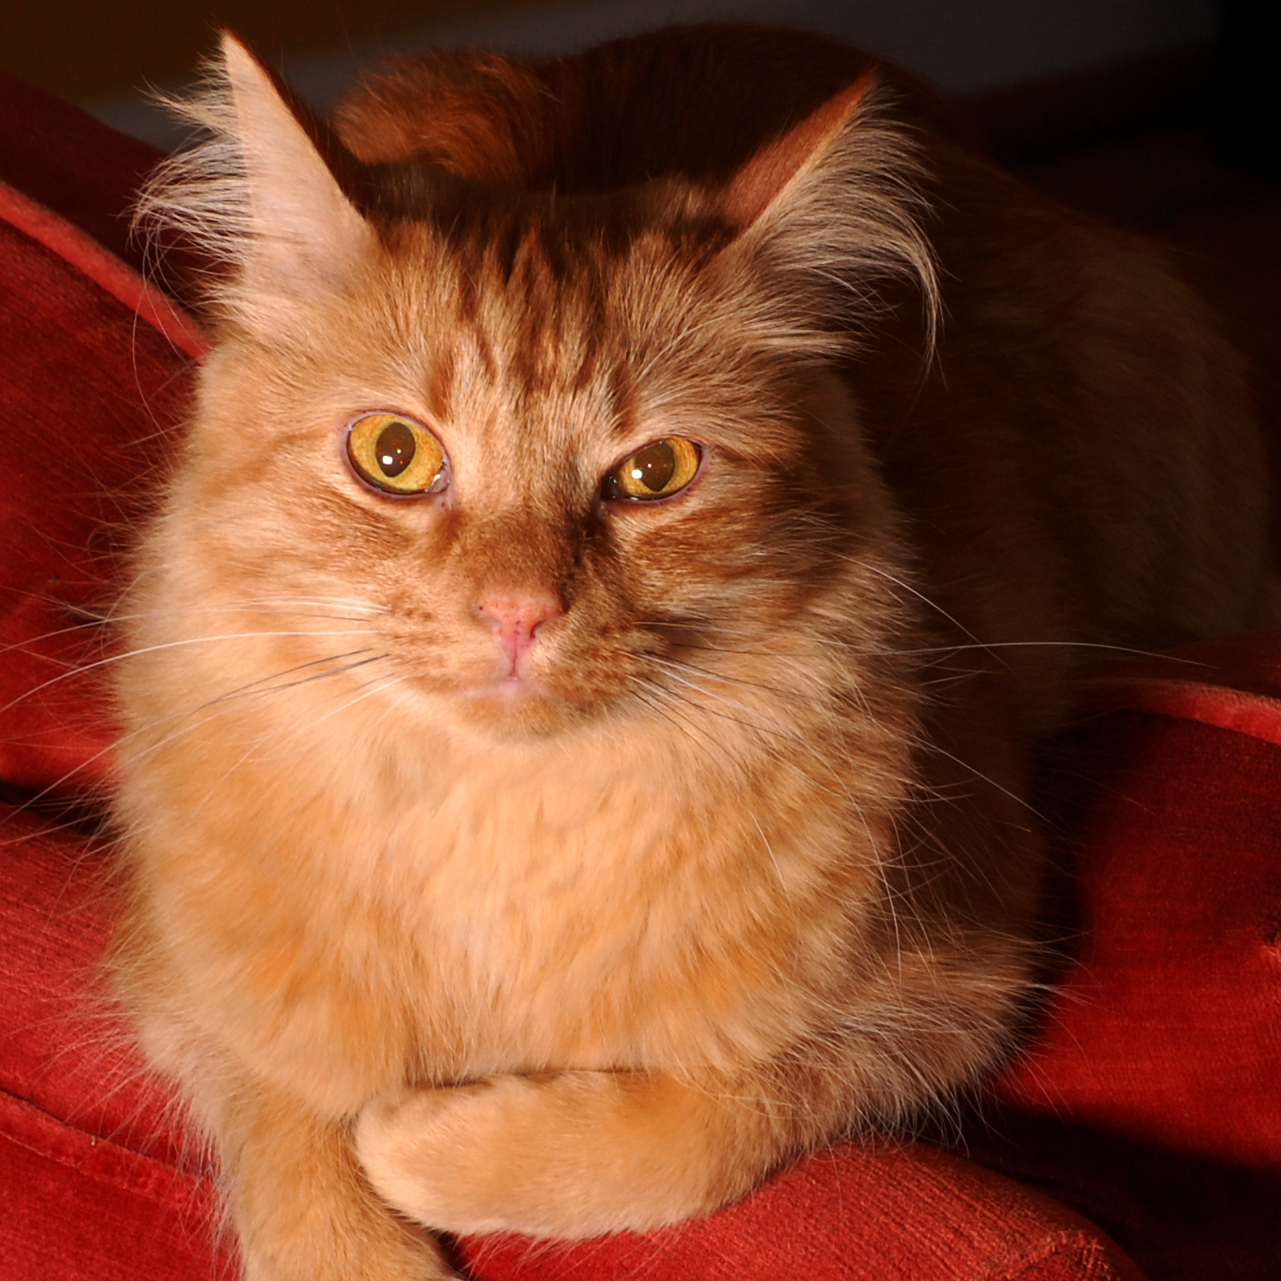
\includegraphics[width=1.5in]{fritz}
\caption{This figure has a caption.}
\label{fig:f1}
\end{center}
\end{figure}

Duis dignissim iaculis mattis. Quisque at sapien est. Proin euismod, metus faucibus sodales blandit, ligula tortor pharetra nisi, commodo suscipit magna nulla sodales purus. In nec quam id nisi suscipit suscipit. Vivamus rutrum bibendum porta. Morbi vestibulum tincidunt dui et sollicitudin. Morbi ut ullamcorper lectus. Mauris non porttitor elit. Ut scelerisque metus et nisi cursus condimentum mattis arcu facilisis. Maecenas ullamcorper porta lobortis. Aliquam erat volutpat. Phasellus sit amet pretium lorem. Aliquam erat volutpat.

\section{Section 3}
Praesent eu nisi vel leo vulputate laoreet. Quisque sit amet venenatis lectus. In augue mauris, mattis et malesuada at, hendrerit et sapien. Nam felis quam, semper in tempus vitae, porttitor a justo. Fusce porta interdum lectus, suscipit molestie felis ultricies at. Vestibulum varius augue elementum nulla congue egestas. Quisque ut lectus vitae tortor hendrerit porta. In congue ultricies elementum. Nulla volutpat neque nec quam mollis cursus. Aenean sapien justo, imperdiet et vulputate a, aliquet sit amet elit. Proin massa orci, blandit non lobortis ac, pretium at arcu. Vivamus sit amet imperdiet eros. Vivamus eget tincidunt nulla. Integer euismod imperdiet libero, sed pellentesque erat ullamcorper quis. Fusce id purus quis dui tristique tristique eget id metus.

\end{document}
